\documentclass[12pt]{article}
\usepackage[czech]{babel}
\usepackage{natbib}
\usepackage{url}
\usepackage[utf8x]{inputenc}
\usepackage{amsmath}
\usepackage{graphicx}
\graphicspath{{images/}}
\usepackage{parskip}
\usepackage{fancyhdr}
\usepackage{vmargin}
\setmarginsrb{3 cm}{2.5 cm}{3 cm}{2.5 cm}{1 cm}{1.5 cm}{1 cm}{1.5 cm}
\usepackage{fancyhdr}
\usepackage{caption}
\usepackage{array}
\newcolumntype{?}[1]{!{\vrule width #1}}
\usepackage{hyperref}
\hypersetup{
    colorlinks=true,
    linkcolor=red,
    filecolor=red,
    urlcolor=blue,
    citecolor=red,
    linktoc=none
    }


\makeatletter
\let\thetitle\@title


\makeatother

\pagestyle{fancy}
\fancyhf{}
\rhead{\theauthor}
\lhead{\thetitle}
\cfoot{\thepage}


%%%%%%%%%%%%%%%%%%%%%%%%%%%%%%%%%%%%%%%%%%%%%%%%%%%%%%%%%%%%%%%%%%%%%%%%%%%%%%%%%%%%%%%%%
\begin{titlepage}
	\centering
    
\includegraphics[scale = 0.35]{FIT_logo.png}\\[1.0 cm]	% University Logo
    \textsc{\LARGE Projektová dokumentace} \\[2.0 cm]
    \textsc{\LARGE Implementace systému pro získání, zpracování a ukládání dat} \\[1 cm]
    \textbf{\LARGE COVID-19}
	\rule{\linewidth}{0.2 mm} \\[0.4 cm]
	{ \huge \bfseries \thetitle}\\

	\vspace{1 cm}
	\begin{minipage}{0.45\textwidth}

            \newline
			\begin{flushleft}
			\emph{Autoři:} \\
			\textbf{Tomáš Beránek (xberan46)} \linebreak
			\textbf{Daniel Kamenický (xkamen21)} \linebreak
			\textbf{Richard Klem (xklemr00)} \linebreak

			% Your Student Number
		    \end{flushleft}
	\end{minipage}\\[0 cm]

    \vspace{8 cm}
    \begin{flushleft}
        Datum odevzdání:\hspace{2 cm}\textbf{16. prosince 2021} \linebreak
    \end{flushleft}

	\vfill
    \fancyhf{}
    \fancyhead[R]{3. listopadu 2021}
\end{titlepage}

%%%%%%%%%%%%%%%%%%%%%%%%%%%%%%%%%%%%%%%%%%%%%%%%%%%%%%%%%%%%%%%%%%%%%%%%%%%%%%%%%%%%%%%%%

\renewcommand{\contentsname}{Obsah}
\tableofcontents
\pagebreak

%%%%%%%%%%%%%%%%%%%%%%%%%%%%%%%%%%%%%%%%%%%%%%%%%%%%%%%%%%%%%%%%%%%%%%%%%%%%%%%%%%%%%%%%%
\begin{document}
\afterpage{\cfoot{\thepage }}

\section{Řešení 2. části projektu}
Cílem 2. části projektu je:
\begin{itemize}
    \item extrakce uložených dat z MongoDB do CSV souborů,
    \item úprava dat pro tvorbu popisných charakteristik a úloh pro dolování z dat.
\end{itemize}

\section{Volba dotazů ze zadání}
\label{dotazy}
Pro vhodné předzpracování dat je dobré znát způsob, jakým se budou data využívat. Na základě této informace je pak možné například -- identifikovat nepotřebná data, která lze v předzpracování odstranit, zvolit vhodný databázový systém, upravit formát atributů v předzpracování atp. Cílem 2. části projektu je realizace dvou dotazů typu A, jednoho dotazu typu B, dvou vlastních dotazů a příprava dat pro jednu z dolovacích úloh typu C.

\textbf{Vybrané dotazy typu A}:
\begin{itemize}
    \item[1)] Vytvořte čárový (spojnicový) graf zobrazující vývoj covidové situace po měsících pomocí následujících hodnot: počet nově nakažených za měsíc, počet nově vyléčených za měsíc, počet nově hospitalizovaných osob za měsíc, počet provedených testů za měsíc. Pokud nebude výsledný graf dobře čitelný, zvažte logaritmické měřítko, nebo rozdělte hodnoty do více grafů.

    \item[] \textbf{Potřebná data}:
    \begin{itemize}
        \item \textbf{počet nově nakažených} (minimální granularita -- měsíc)
        \item \textbf{počet nově vyléčených} (minimální granularita -- měsíc)
        \item \textbf{počet nově hospitalizovaných} (minimální granularita -- měsíc)
        \item \textbf{počet nově provedených testů} (minimální granularita -- měsíc)
    \end{itemize}

    \hspace{1cm}

    \item[3)] Vytvořte sérii sloupcových grafů, které zobrazí:
    \begin{itemize}
        \item počty provedených očkování v jednotlivých krajích (celkový počet od začátku očkování),
        \item počty provedených očkování jako v předchozím bodě navíc rozdělené podle pohlaví. Diagram může mít např. dvě části pro jednotlivá pohlaví,
        \item počty provedených očkování, ještě dále rozdělené dle věkové skupiny. Pro potřeby tohoto diagramu postačí 3 věkové skupiny (0-24 let, 25-59 let, nad~59).
    \end{itemize}

    \item[] \textbf{Potřebná data}:
    \begin{itemize}
        \item \textbf{počet provedených očkovaní u můžu/žen v daném kraji} (minimální granularita -- celkem)
        \item \textbf{počet provedených očkovaní podle věku v daném kraji} (minimální granularita počtu očkování -- celkem, minimální granularita věku -- 0-24 let, 25-59 let a nad 59 let)
    \end{itemize}
\end{itemize}

\hspace{1cm}

\textbf{Vybraný dotaz typu B}:
\begin{itemize}
    \item[2)] Vytvořte sérii sloupcových grafů (alespoň 3), které porovnají vývoj různých covidových ukazatelů vámi zvoleného kraje se zbytkem republiky. Jako covidové ukazatele můžete použít: počet nakažených osob, počet hospitalizovaných osob, počet zemřelých, počet očkovaných. Všechny hodnoty uvažujte přepočtené na jednoho obyvatele kraje/republiky. Zobrazte alespoň 12 po sobě jdoucích hodnot (např. hodnoty za poslední rok po měsících).
\end{itemize}

    \item[] \textbf{Potřebná data}:
    \begin{itemize}
        \item \textbf{celkový počet nakažených podle kraje} (minimální granularita -- měsíc)
        \item \textbf{celkový počet zemřelých podle kraje} (minimální granularita -- měsíc)
        \item \textbf{celkový počet očkovaných podle kraje} (minimální granularita -- měsíc)
    \end{itemize}

\hspace{1cm}

\textbf{Vlastní dotazy} zahrnující data alespoň ze dvou zdrojů:
\begin{itemize}
    \item[1)] Vytvořte sloupcový graf rozdělený podle věku (po 5letých intervalech) obyvatelstva ve vybraném okresu. Každý sloupec vyjadřuje kolik procent obyvatelstva z dané věkové skupiny dostalo COVID-19 za poslední rok (neuvažujte duplicity).

    \item[] \textbf{Potřebná data}:
    \begin{itemize}
        \item \textbf{počet nakažených podle věku a okresu} (minimální granularita věku -- 5leté intervaly)
        \item \textbf{počet obyvatel podle věku a okresu} (minimální granularita věku -- 5leté intervaly)
    \end{itemize}

    \item[2)] Vytvořte graf, který ukazuje vývoj počtu nakažených žen a mužů začátku pandemie COVID-19 po měsících. Hodnoty uvádějte v procentech (např. 100\% u mužů znamená, že jsou nakaženi všichni muži).

    \item[] \textbf{Potřebná data}:
    \begin{itemize}
        \item \textbf{počet nakažených podle pohlaví } (minimální granularita -- měsíc)
    \end{itemize}
\end{itemize}

\hspace{1cm}

\textbf{Vybraná dolovací úloha typu C}:
\begin{itemize}
    \item[1)] Hledání skupin podobných okresů z hlediska vývoje covidu a věkového složení obyvatel.
    \begin{itemize}
        \item Atributy: počet nakažených za poslední 4 čtvrtletí, počet očkovaných za poslední 4 čtvrtletí, počet obyvatel ve věkové skupině 0..14 let, počet obyvatel ve věkové skupině 15 - 59, počet obyvatel nad 59 let.
        \item Pro potřeby projektu vyberte libovolně 50 okresů, pro které najdete potřebné hodnoty (můžete např. využít nějaký žebříček 50 nejlidnatějších okresů v ČR).
    \end{itemize}

    \item[] \textbf{Potřebná data}:
    \begin{itemize}
        \item \textbf{počet nakažených podle věku a okresů} (minimální granularita věku -- 0-24 let, 25-59 let a nad 59 let, minimální granularita datumu -- 3 měsíce)
        \item \textbf{počet očkovaných podle věku a okresů} (minimální granularita věku -- 0-24 let, 25-59 let a nad 59 let, minimální granularita datumu -- 3 měsíce)
        \item \textbf{počty obyvatel v jednotlivých okresech podle věku} (minimální granularita věku -- 0-24 let, 25-59 let a nad 59 let)
    \end{itemize}
\end{itemize}

\newpage
\section{Extrahování dat z MongoDB do CSV souborů}
Pro spuštění tohoto kroku je nutné mít vytvořenou a naplněnou databázi z 1. části projektu. Podrobný popis vkládání dat do databáze je uveden v dokumentaci 1. části projektu, která je umístěna v kořenové složce adresáře. Extrahování dat zajišťuje Python3 skript \texttt{src/mongo\_to\_dataframe.py}. Obdobně jako v 1. části je zde využito knihovny \texttt{pymongo}. Skript generuje CSV soubory do složky \texttt{data-part2/}. Každý soubor má prefix \texttt{A1}, \texttt{A3}, \texttt{B2}, \texttt{V1}, \texttt{V2} nebo \texttt{C1}, který udává pro jaké dotazy bude použit.

\section{Dotaz A1}
Pro tento dotaz byly z databáze extrahovány čtyři soubory:
\begin{itemize}
    \item \texttt{A1-hospitalizace.csv} s atributy:
        \begin{itemize}
            \item \texttt{datum}
            \item \texttt{pocet\_hosp}
        \end{itemize}
    \item \texttt{A1-kraj-okres-testy.csv} s atributy:
        \begin{itemize}
            \item \texttt{datum}
            \item \texttt{prirustkovy\_pocet\_testu\_okres}
        \end{itemize}
    \item \texttt{A1-osoby.csv} s atributy:
        \begin{itemize}
            \item \texttt{datum}
        \end{itemize}
    \item \texttt{A1-vyleceni.csv} s atributy:
        \begin{itemize}
            \item \texttt{datum}
        \end{itemize}
\end{itemize}

U tohoto dotazu (ani u ostatních) není detailně popsána implementace. Je však možno nahlédnout do komentovaných zdrojových kódů v repozitáři. Pro zodpovězení dotazu A1 byl vytvořen obrázek se třemi grafy, viz. obrázek \ref{A1}. První graf ukazuje vývoj počtu nakažených a vyléčených lidí. Jelikož jsou tyto ukazatele velmi podobné (mají podobný průběh), tak byly vloženy do jednoho obrázku. Druhý graf ukazuje vývoj počtu hospitalizovaných. Jelikož jsme neměli k dispozici přírustkový počet hospitalizovaných (pouze aktuální počet), tak měsiční hodnota je vypočítána jako průměr všech dní v daném měsíci. Tento graf byl oddělen, protože počty hospitalizovaných jsou razantně menší a křivka v grafu by se jevila téměř jako přímka u hodnoty 0. Třetí graf ukazuje počet provedených testů. Tento graf byl také oddělen, jelikož počty provedených testů jsou razantně větší než počty v prvním/druhém grafu a docházelo by tak ke změnšení detailu u předchozích ukazatelů.

\begin{center}
    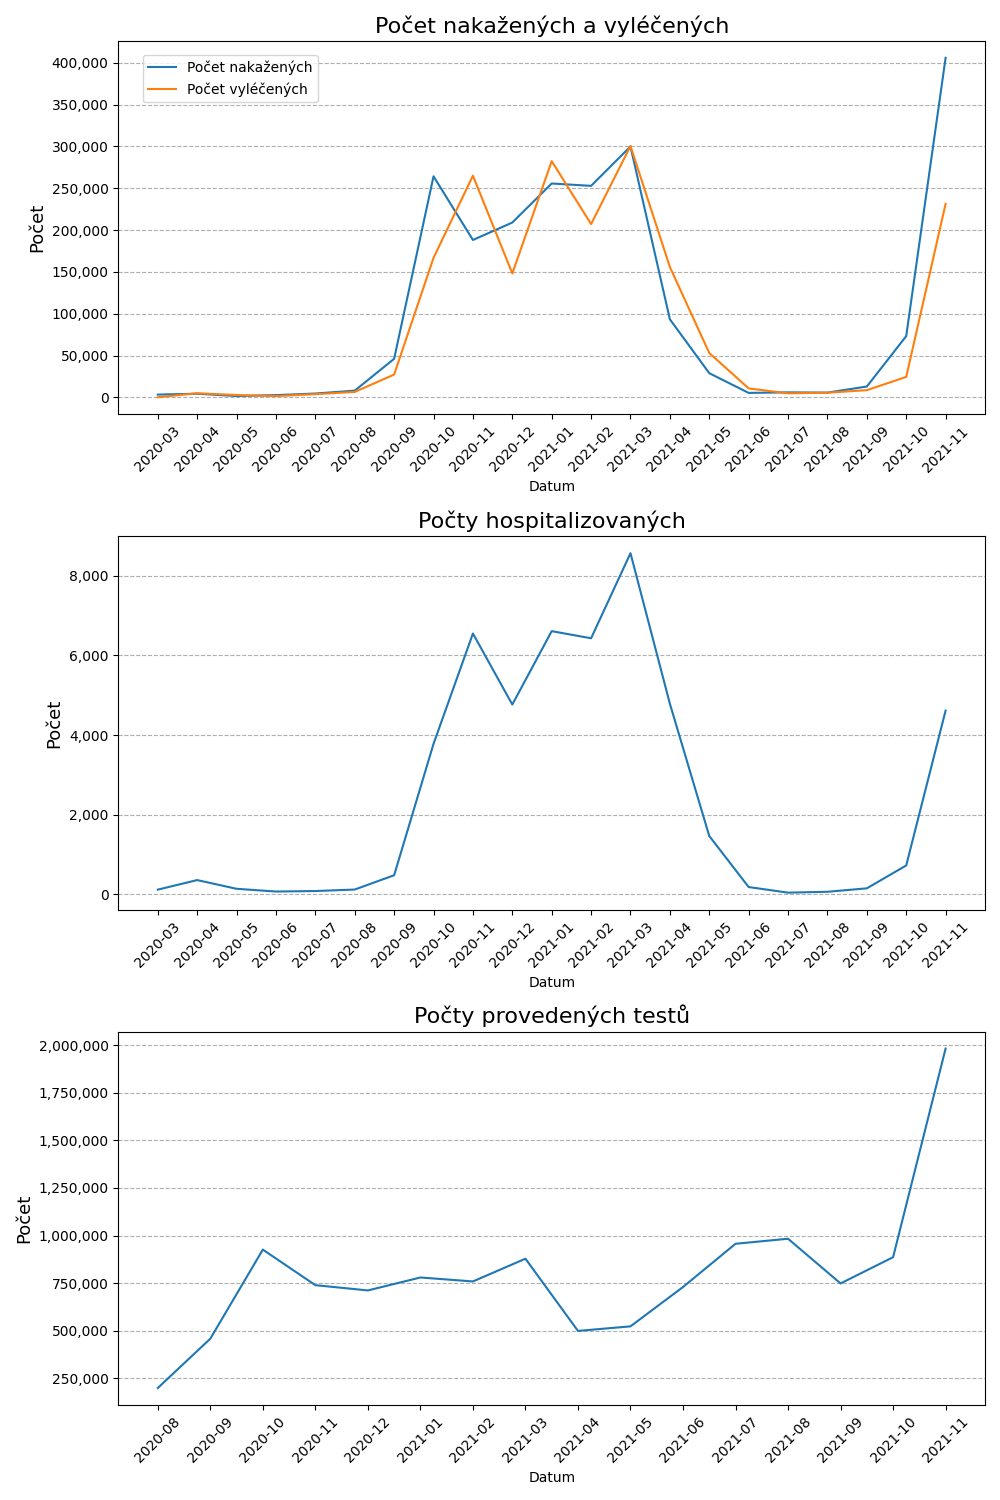
\includegraphics[width=0.63\paperwidth]{A1-vyvoj_situace.png}
    \captionof{figure}{Vizualizace dotazu A1. Graf zobrazující vývoj covidové situace.}
    \label{A1}
\end{center}

\section{Dotaz A3}
Pro zodpovězení dotazu A3 byl z databáze extrahován jeden soubor:
\begin{itemize}
    \item \texttt{A3-\ockovani-profese.csv} s atributy:
        \begin{itemize}
            \item \texttt{datum}
            \item \texttt{vakcina}
            \item \texttt{kraj\_nazev}
            \item \texttt{poradi\_davky}
            \item \texttt{vekova\_skupina}
            \item \texttt{pohlavi}
        \end{itemize}
\end{itemize}

Pro zodpovězení dotazu A3 byly vytvořeny dva obrázky. Obrázek \ref{A3-1} obsahuje grafy, které popisují počty provedených očkování v jednotlivých krajích navíc rozdělené podle pohlaví. Obrázek \ref{A3-2} obsahuje tři grafy, které tyto statistiky rozdělují ještě podle věku.

\begin{center}
    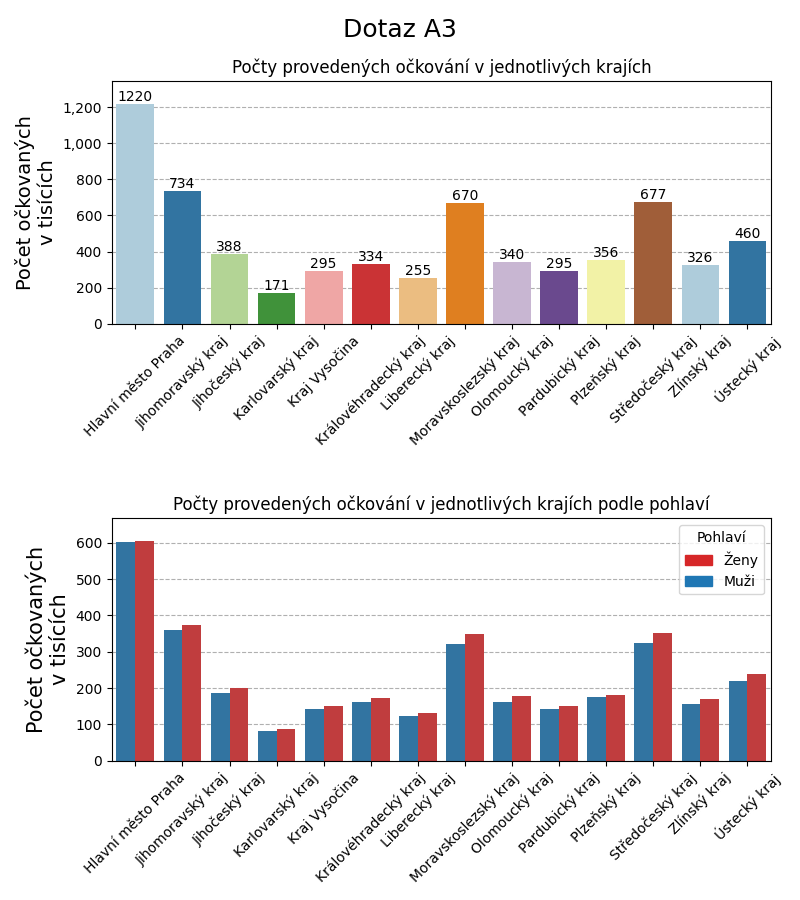
\includegraphics[width=0.7\paperwidth]{A3-kraje-a-pohlavi.png}
    \captionof{figure}{Vizualizace dotazu A3. Počty provedených očkování v jednotlivých krajích navíc rozdělené podle pohlaví.}
    \label{A3-1}
\end{center}


\begin{center}
    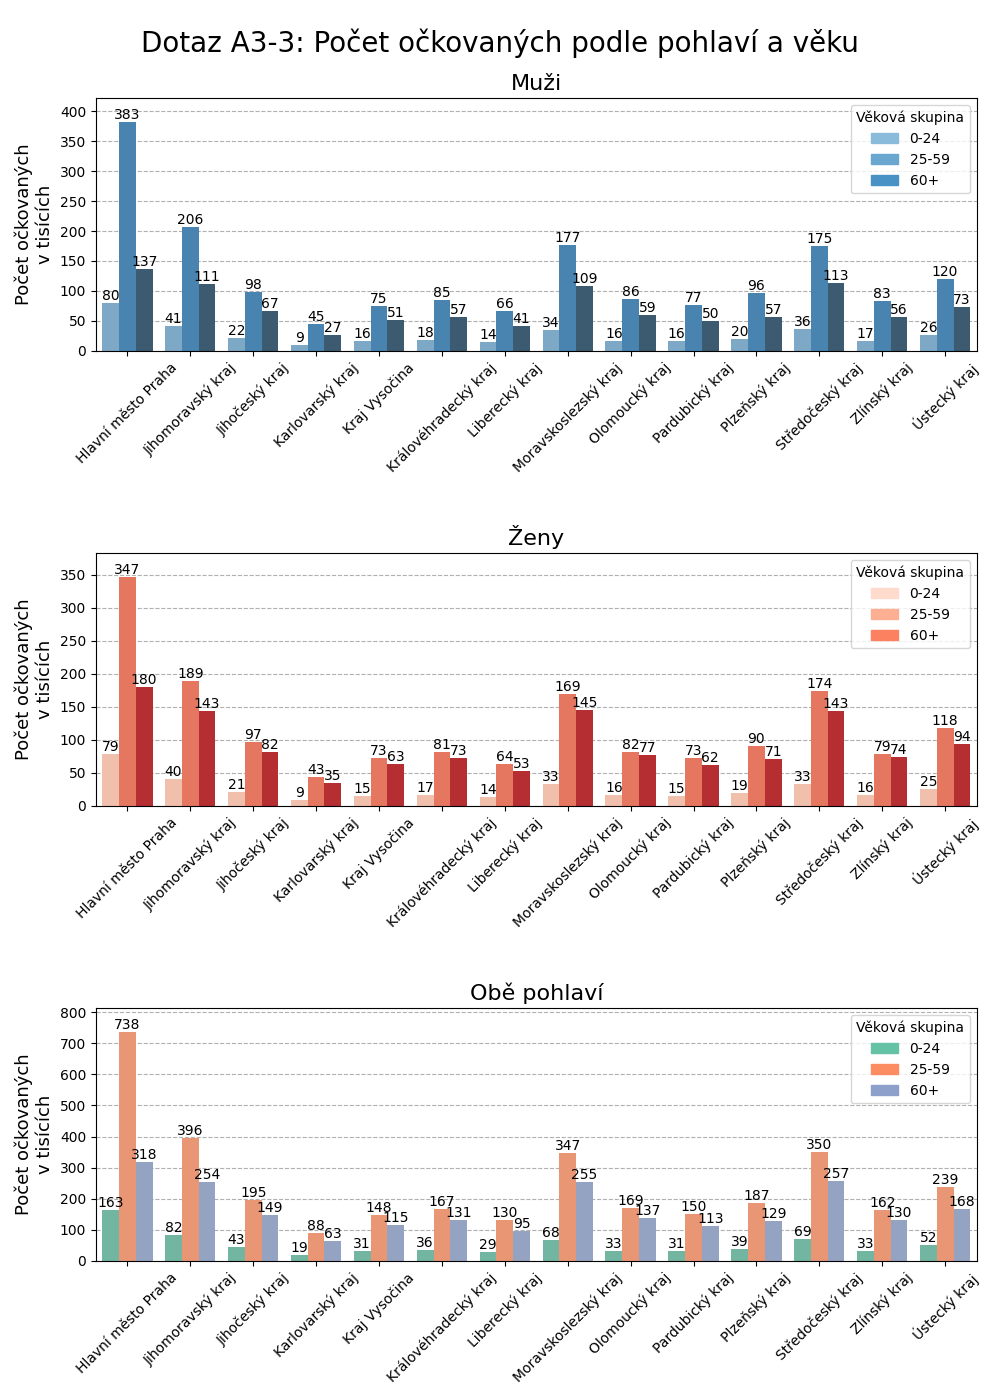
\includegraphics[width=0.63\paperwidth]{A3-pohlavi-a-vek.png}
    \captionof{figure}{Vizualizace dotazu A3. Počty provedených očkování v jednotlivých krajích rozdělené podle pohlaví a podle věku.}
    \label{A3-2}
\end{center}


\section{Dotaz B2}
Pro tento dotaz byly z databáze extrahovány tři soubory:
\begin{itemize}
    \item \texttt{B2-ockovani-profese.csv} s atributy:
        \begin{itemize}
            \item \texttt{datum}
            \item \texttt{vakcina}
            \item \texttt{kraj\_nuts\_kod}
            \item \texttt{poradi\_davky}
        \end{itemize}
    \item \texttt{B2-osoby.csv} s atributy:
        \begin{itemize}
            \item \texttt{datum}
            \item \texttt{kraj\_nuts\_kod}
        \end{itemize}
    \item \texttt{B2-umrti.csv} s atributy:
        \begin{itemize}
            \item \texttt{datum}
            \item \texttt{kraj\_nuts\_kod}
        \end{itemize}
\end{itemize}


Pro zodpovězení dotazu B2 byly vytvořeny tři grafy, které ukazují porovnání Hlavního Města Prahy se zbytkem republiky. První graf porovnává počty nakažených, viz. obrázek \ref{B2-1}. Druhý graf porovnává počty \textbf{plně} očkovaných, viz. obrázek \ref{B2-2}. A třetí graf porovnává počty úmrtí, viz. obrázek~\ref{B2-3}.

\begin{center}
    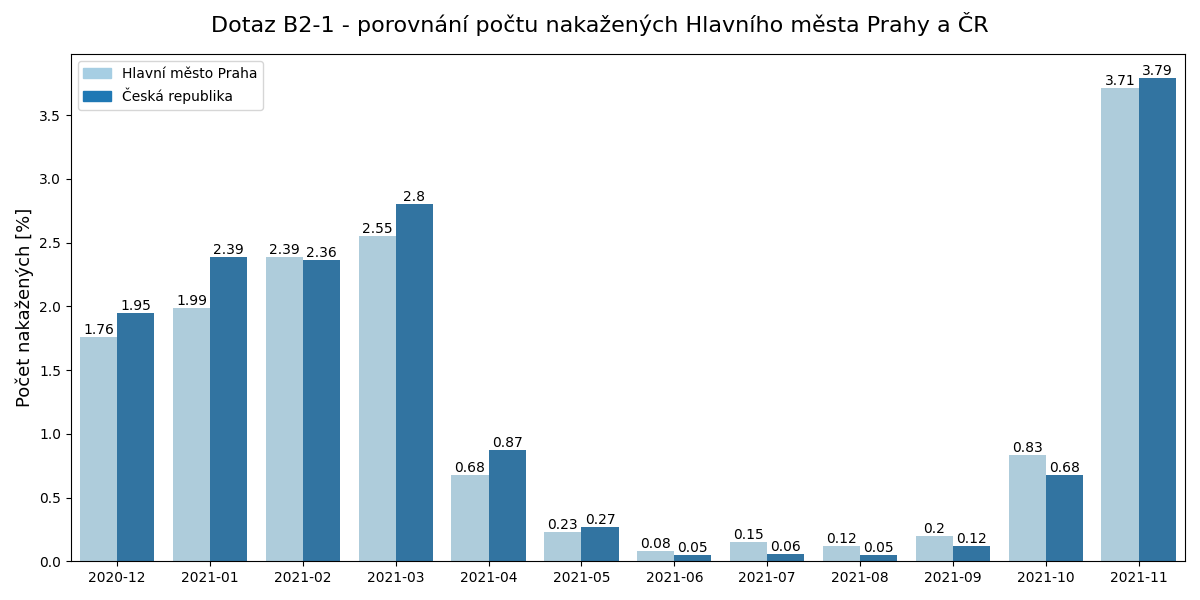
\includegraphics[width=0.7\paperwidth]{B2-nakazeni.png}
    \captionof{figure}{Vizualizace dotazu B2. Porovnání počtu nakažených.}
    \label{B2-1}
\end{center}

\begin{center}
    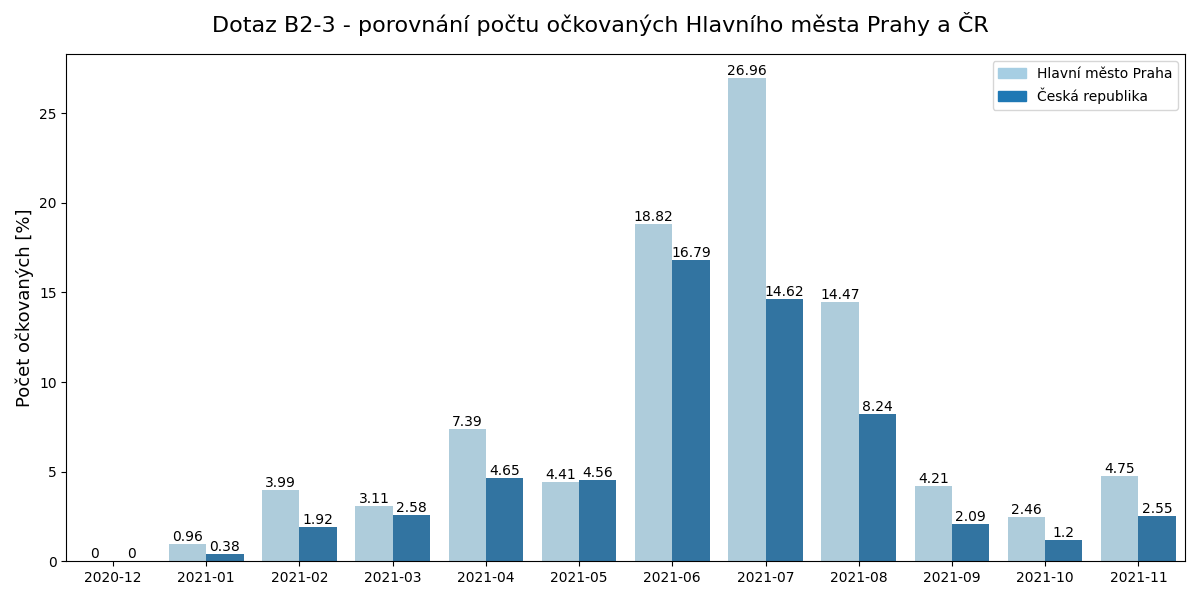
\includegraphics[width=0.7\paperwidth]{B2-ockovani.png}
    \captionof{figure}{Vizualizace dotazu B2. Porovnání počtu očkovaných.}
    \label{B2-2}
\end{center}

\begin{center}
    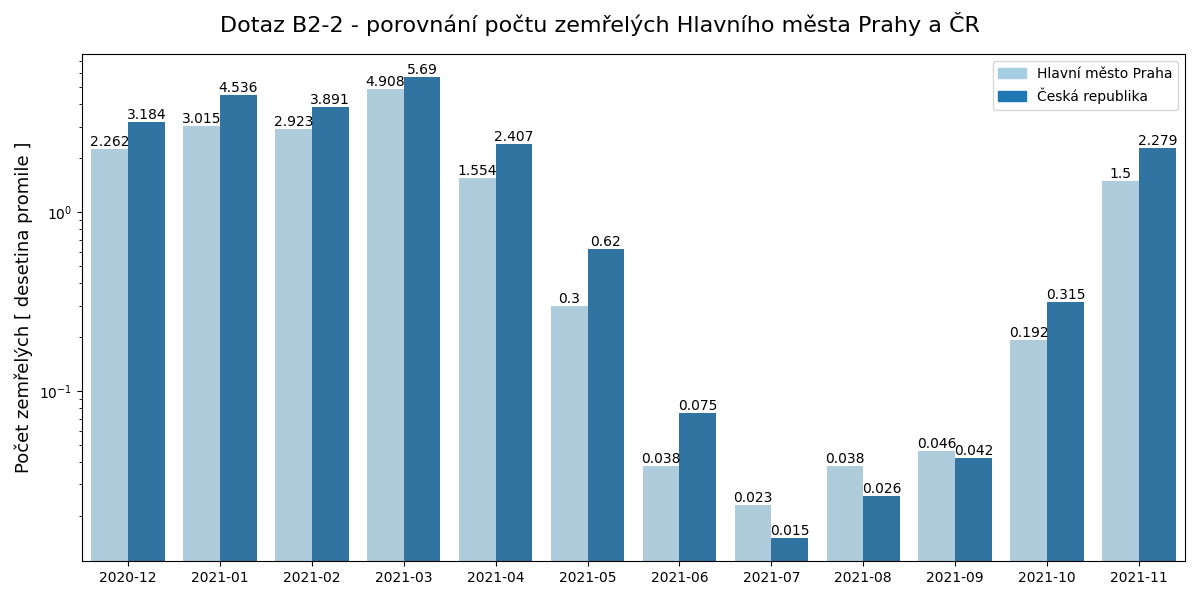
\includegraphics[width=0.7\paperwidth]{B2-zemreli.png}
    \captionof{figure}{Vizualizace dotazu B2. Porovnání počtu úmrtí.}
    \label{B2-3}
\end{center}

\newpage
\section{Dotaz V1}
Pro tento dotaz byly z databáze extrahovány tři soubory:
\begin{itemize}
    \item \texttt{V1-130142-21data043021.csv} s atributy:
        \begin{itemize}
            \item \texttt{hodnota}
            \item \texttt{vek\_txt}
            \item \texttt{vuzemi\_txt}
            \item \texttt{casref\_do}
            \item \texttt{pohlavi\_kod}
        \end{itemize}
    \item \texttt{V1-obce.csv} s atributy:
        \begin{itemize}
            \item \texttt{okres\_lau\_kod}
            \item \texttt{okres\_nazev}
        \end{itemize}
    \item \texttt{V1-osoby.csv} s atributy:
        \begin{itemize}
            \item \texttt{datum}
            \item \texttt{vek}
            \item \texttt{okres\_lau\_kod}
        \end{itemize}
\end{itemize}
Pro zodpovězení dotazu V1 byl vytvořen graf, který ukazuje zastoupení nakažených ve věkových skupinách v okresu Opava za poslední rok, viz. obrázek \ref{V1}.

\begin{center}
    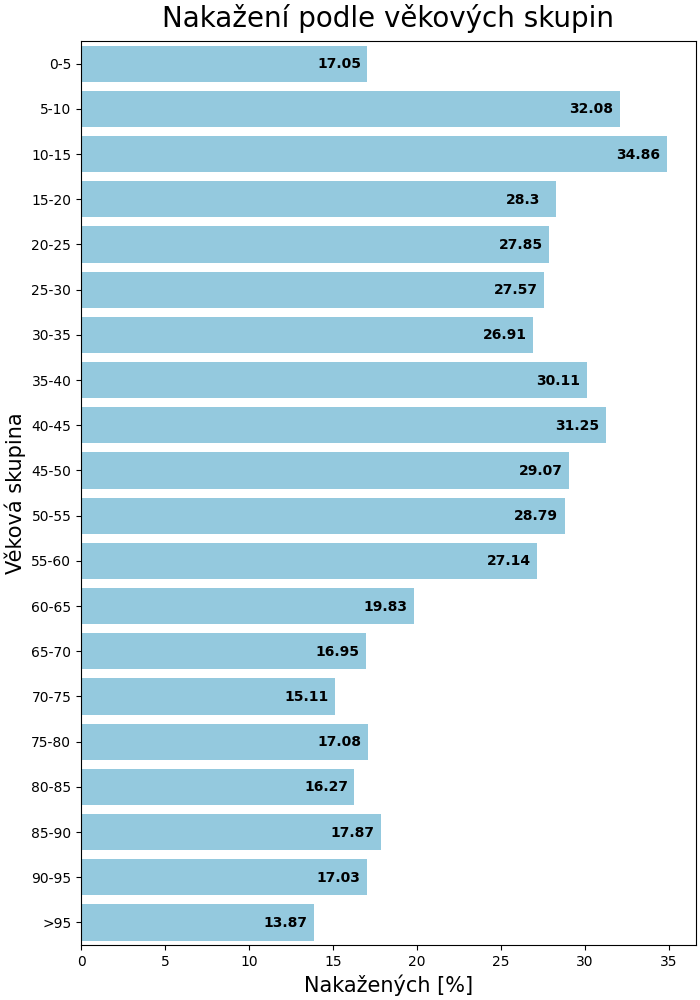
\includegraphics[width=0.63\paperwidth]{V1-nakazenych-podle-veku.png}
    \captionof{figure}{Vizualizace dotazu V1. Zastoupení nakažených ve věkových skupinách v okresu Opava za poslední rok.}
    \label{V1}
\end{center}

\section{Dotaz V2}
Pro tento dotaz byl z databáze extrahován jeden soubory:
\begin{itemize}
    \item \texttt{V2-osoby.csv} s atributy:
        \begin{itemize}
            \item \texttt{datum}
            \item \texttt{pohlavi}
        \end{itemize}
\end{itemize}

Pro zodpovězení dotazu V2 byl vytvořen graf, který ukazuje procentuální zastoupení nakažených můžu/žen, viz. obrázek \ref{V2}. Tento dotaz jsme zvolili, abychom zjistili, zda je některé pohlaví náchylnější na nakažení.

\begin{center}
    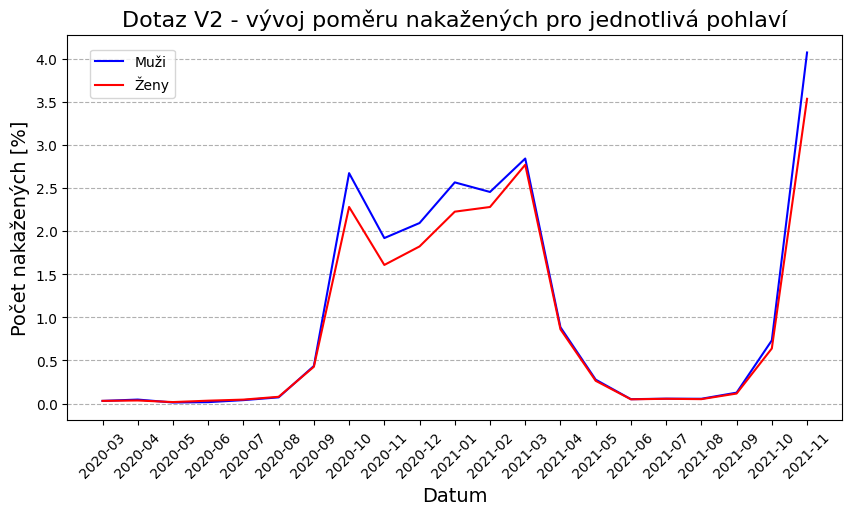
\includegraphics[width=0.7\paperwidth]{V2-nakazeni.png}
    \captionof{figure}{Vizualizace dotazu V2. Graf procentuálního zastoupení nakažených mezi muži/ženami.}
    \label{V2}
\end{center}

\section{Dotaz C1}
Pro tento dotaz byly z databáze extrahovány čtyři soubory:
\begin{itemize}
    \item \texttt{C1-130142-21data043021.csv} s atributy:
        \begin{itemize}
            \item \texttt{hodnota}
            \item \texttt{pohlavi\_kod}
            \item \texttt{casref\_do} -- datum, ke kterému řádek platil
            \item \texttt{vek\_txt}
            \item \texttt{vuzemi\_txt} -- ČR, kraje a okresy
        \end{itemize}
    \item \texttt{C1-obce.csv} s atributy:
        \begin{itemize}
            \item \texttt{okres\_lau\_kod}
            \item \texttt{okres\_nazev}
            \item \texttt{orp\_kod}
        \end{itemize}
    \item \texttt{C1-ockovani-profese.csv} s atributy:
        \begin{itemize}
            \item \texttt{datum}
            \item \texttt{vakcina}
            \item \texttt{kraj\_nuts\_kod}
            \item \texttt{poradi\_davky}
            \item \texttt{vekova\_skupina}
            \item \texttt{orp\_bydliste\_kod}
        \end{itemize}
    \item \texttt{C1-osoby.csv} s atributy:
        \begin{itemize}
            \item \texttt{datum}
            \item \texttt{okres\_lau\_kod}
        \end{itemize}
\end{itemize}

Výsledkem tohoto dotazu je CSV soubor \texttt{data-mining/C1-data.csv} s následujícími atributy:
        \begin{itemize}
            \item \texttt{okres\_nazev} -- název okresu. Bylo vybráno 50 nejlidnatějších okresů v ČR. Do těchto okresů počítáme i Hlavní Město Prahu, ikdyž se technicky vzato nejedná o okres, ale o kraj. Nicméně jsme chtěli vidět statistiky z Prahy.
            \item \texttt{4\_nakazeni} -- počet nakažených za poslední kvartál. Hodnota v tomto sloupci byla nejdříve transformována na počet nakažených na 1000 obyvatel daného okresu. Poté byly odstraněny odlehlé hodnoty pomocí IQR a nahrazeny průměrnou hodnotou (bez odlehlých hodnot). Nakonec byla tato hodnota normalizována pomocí metody min-max do intervalu 0 až 1.
            \item \texttt{3\_nakazeni} -- počet nakažených za předposlední kvartál. ...
            \item \texttt{2\_nakazeni} -- ...
            \item \texttt{1\_nakazeni} -- ...
            \item \texttt{4\_ockovani} -- počet očkovaných za poslední kvartál. Hodnota v tomto sloupci byla opět nejdříve přepočtena na 1000 obyvatel daného kraje, opět byly obdobně odstraněny a nahrazeny odlehlé hodnoty. Poté se obdobně provedla normalizace a nakonec diskretizace těchto hodnot do tří kategorií, které udávají jaká je proočkovanost daného okresu vůči ostatním okresům za daný kvartál:
                \begin{itemize}
                    \item \texttt{nízká} -- hodnoty od 0 (včetně) do 0.3.
                    \item \texttt{střední} -- hodnoty od 0.3 (včetně) do 0.7.
                    \item \texttt{vysoká} -- hodnoty od 0.7 (včetně) do 1 (včetně).
                \end{itemize}
            \item \texttt{3\_ockovani} -- počet očkovaných za předposlední kvartál. ...
            \item \texttt{2\_ockovani} -- ...
            \item \texttt{1\_ockovani} -- ...
            \item \texttt{0\_14\_vek} -- počet obyvatel okresu ve věku 0 (včetně) až 14 let.
            \item \texttt{15\_59\_vek} -- počet obyvatel okresu ve věku 15 (včetně) až 59 let.
            \item \texttt{60\_vek} -- počet obyvatel okresu ve věku 60 a více let.
        \end{itemize}
        
Ve sloupci \texttt{3\_nakazeni} bylo odstraněno 5 odlehlých hodnot, ve sloupci \texttt{1\_nakazeni} byly odstraněny 3 hodnoty a ve sloupci \texttt{1\_ockovani} byla odstraněna 1 hodnota.

CSV soubor \texttt{data-mining/C1-data-bez-uprav.csv} obsahuje neupravená (tzn. bez transformace, normalizace, diskretizace a odstranění odlehlých hodnot) data pro data miningovou úlohu.

\section{Návod na spuštění}
Prerekvizity, specifické vlastnosti chování, potřebná nastavení a návod na spuštění jsou popsány v dokumentaci v souboru \texttt{README.md}, který je umístěn v kořenovém adresáři projektu. Celý projekt (1. i 2. část) funguje jako jedna pipeline -- stáhne data, transformuje na JSON, vyfiltruje, vloží do Mongo DB, extrahuje do CSV, vygeneruje grafy a vytvoří CSV pro data mining. Jelikož je ve WISu limit na 10MB a naše extrahovaná CSV data mají přibližně 2GB, tak jsou data ke stažení \href{https://drive.google.com/drive/folders/1RmdLxXcsgwmM98bOfyiooRcAh_S5xCwm?usp=sharing}{na této adrese}. Stažená data vložte i se složkou \texttt{data-part2/} do kořenového adresáře repozitáře.

Při vytváření grafů, skript ukládá do složky \texttt{dumps/} CSV soubory, které obsahují data, ze kterých jsou grafy vygenerovány.

\end{document}
